\chapter{Umsetzung des Datentransformations- und Verteilungssystems}

Die Hauptaufgaben dieses Werkzeuges ist die Gewinnung der Daten aus den verschiedenen Diensten. Diese Daten werden dann in einer Datenbank gespeichert und können bei einer Abfrage zur Übertragung in einen anderen Dienst verändert werden. Zur Ermöglichung dieses Ziels müssen die Unterschiedlichen Informationen aus den Anwendungen auf eine gemeinsame Datenmenge zusammengeführt werden. Darauf folgt die Festlegung der Klassenstruktur, eine Definition des Speichervorganges in die Datenbank und die Umsetzung der Rückführung in den selben oder einen anderen Dienst. Das Projekt fokussiert sich auf Dienstleister in den Bereichen Kalender- und Notiz-Verwaltung, wobei zu jedem Bereich jeweils drei Angebote eingebunden werden. Die Notiz-Verwaltung, auf welche sich diese Arbeit hauptsächlich konzentriert, wird dabei von \textit{Keep} (Google), \textit{OneNote} (Microsoft) und \textit{Notion} (Notion) vertreten.

\section{Zusammenführung der Daten}

Als erster Schritt werden die Daten aus den verschiedenen Schnittstellen aufgelistet. Dafür werden alle möglichen Attribute, welche man aus den Diensten extrahieren kann, in einer Liste gesammelt und diese mit den Eigenschaften der anderen Dienste verglichen. Gibt es Übereinstimmungen in Bezeichnung oder Funktion, wir dieses Attribut für das gemeinsame Datenformat akzeptiert. Unter den gemeinsamen Daten gibt es dabei rein informative Informationen, wie beispielsweise den Titel oder einen Text, sowie für die Funktion des Dienstes strukturell notwendige Werte, wie die ID. Diese sind zwar für jede Anwendung vorhanden, unterscheiden sich allerdings nahezu jedes mal in ihren Werten. Bei der Verwendung dieser als gemeinsames Attribut muss noch eine Anpassung der Werte vorgenommen werden. Der Vorgang ist für die Notiz-Anwendungen in Abbildung \ref{fig:attrMatch} zu sehen.\\

\begin{figure}[H]
	\centering
	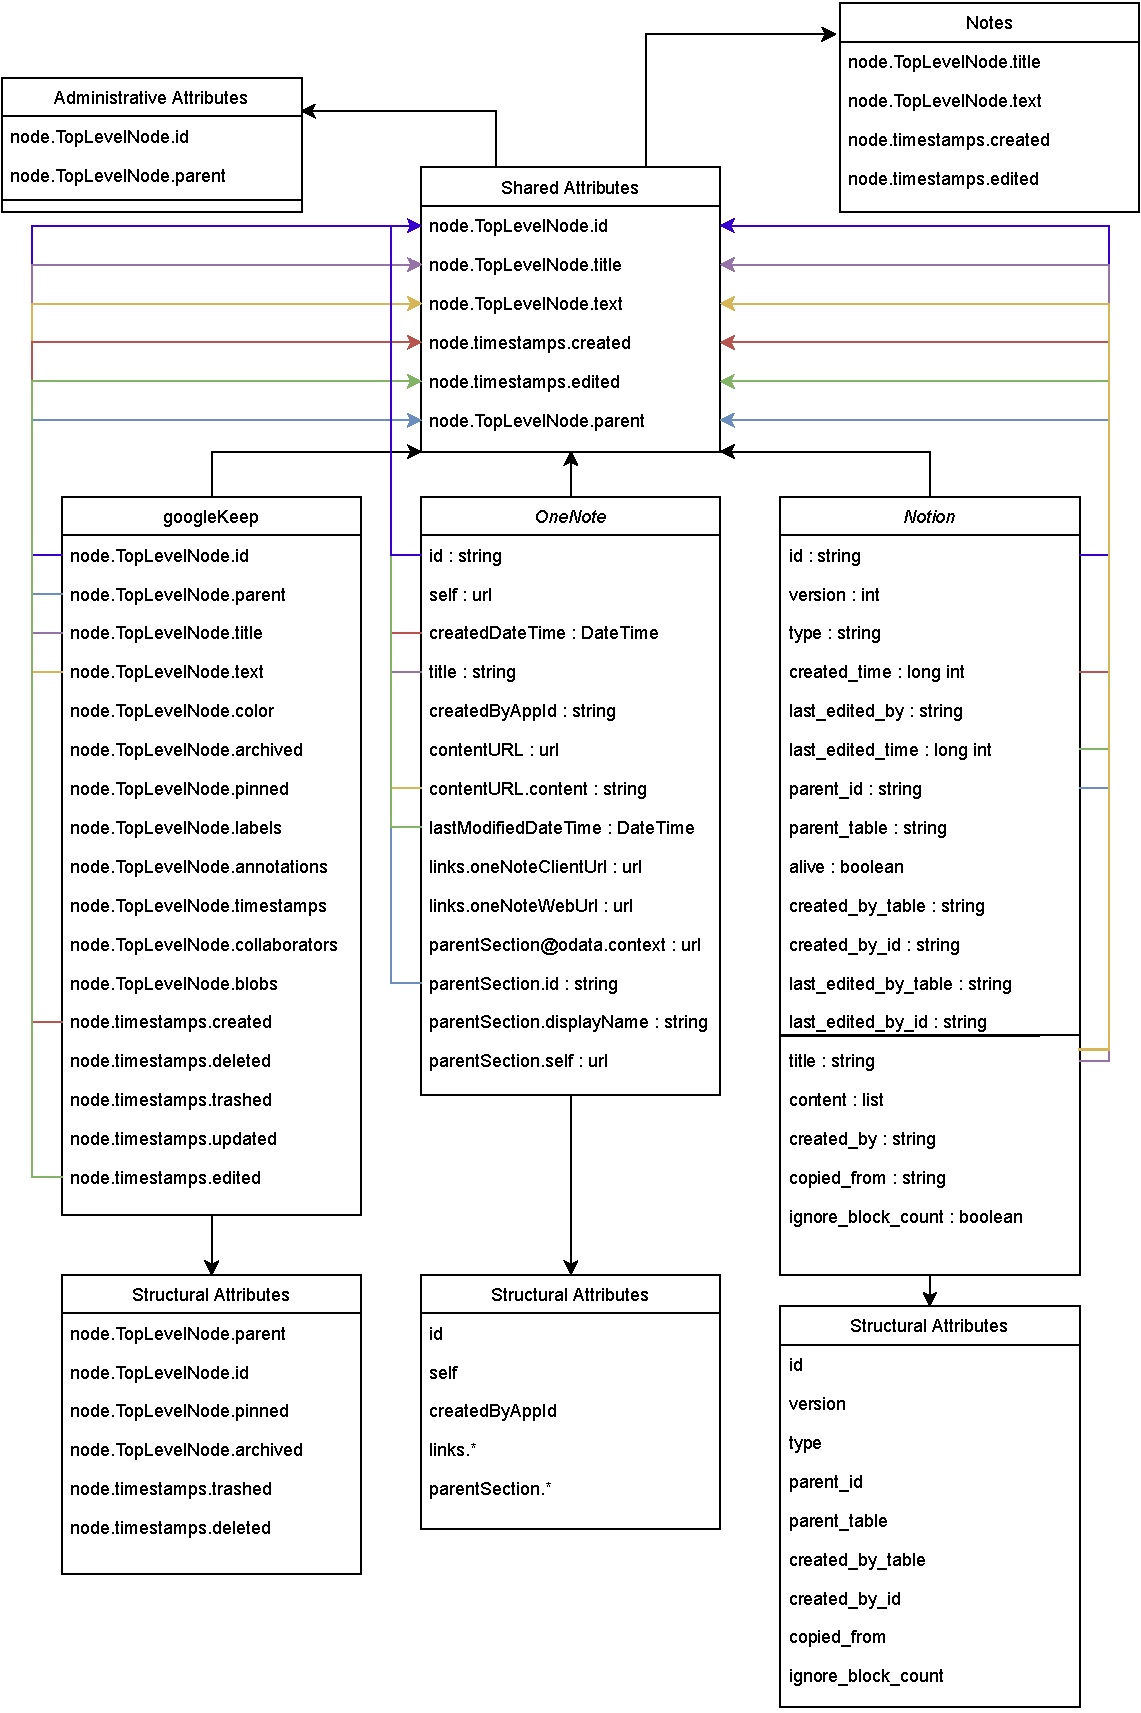
\includegraphics[width=1\textwidth]{Bilder/umsetzung/attributeUnion.pdf}
	\caption{Darstellung des Attribut-Vereinigungsprozesses}
	\label{fig:attrMatch}
\end{figure}
\clearpage

Nach der Vereinigung dieser Attribute mit denen aus den Kalender-Diensten, wurden folgende Attribute in Tabelle \ref{tab:daten} für als feste, zwingend notwendige Eigenschaften eines internen Datensatzes definiert. \\

\begin {table}[H]
	\caption{Gemeinsame Attribute aller Dienste}
	\begin{tabular}{|l|l|l|}
		\hline
		Wert & Datentyp & besondere Formatierung\\
		\hline
		id & string & <Diensttyp>\#<Dienstklassenname>\#<Dienst-ID>\\
		title & string & \\
		text & string & \\
		created & string & <J>-<M>-<T>T<S>:<M>:<S>.<ZZ> (UTC-Zeitformat)\\
		edited & string & <J>-<M>-<T>T<S>:<M>:<S>.<ZZ> (UTC-Zeitformat)\\
		\hline
	\end{tabular}
	\label{tab:daten}
\end{table}

Jeder Datensatz aus den Anwendungen muss diese Attribute enthalten, um in die Datenbank aufgenommen zu werden. Die übrigen Eigenschaften, welche nicht in allen anderen Diensten enthalten sind, werden ebenfalls in die Datenbank übertragen. Bei diesen muss jedoch bei der Rückführung in den Dienst die Existenz geprüft werden. \\

\section{Festlegung der Klassenstruktur}

Um sicherzustellen, dass die festen Attribute vorhanden sind, werden die Daten in einer Klasse gespeichert. Dabei gibt es eine Basisklasse, welche diese Daten enthält, und mehrere abgeleitete Klassen mit den diensteigenen Werten. Diese Klassen besitzten keine Methoden, da sie als reine Speicherklassen genutzt werden. Objekte dieser Klassen werden durch die Dienst-Schnittstellenklassen erstellt. Ihre Aufgabe ist die Kommunikation mit den Diensten über deren jeweilige Benutzerschnittstellen. Sie übernehmen also die Anmeldung, die Extrahierung von Daten aus der Anwendung und die Injektion der Daten aus der Datenbank zurück in den Dienst. Sie fungieren außerdem als Bedienungsschnittstelle für die Nutzeroberfläche. Dabei werden auch hier alle Dienst-Schnittstellenklassen von einer Basis-Klasse abgeleitet, wodurch man sicherstellt, dass alle Unterklassen auf die gleichen Resourcen zugreifen und die gleiche Funktionalität bereitstellen. Die letzte Klassengruppe stellen die Datenbank-Schnittstellenklassen dar. Diese ermöglichen den Datentransfer zu und von der Datenbank. Ebenso wie bei den Dienst-Klassen, wir auch hier eine Vererbungsstruktur genutzt, um eine Konsistenz zwischen den abgeleiteten Klassen sicherzustellen. Das gesammte Konzept ist dabei auf hohe Flexibilität ausgelegt. So kann ein neuer Dienst einfach über das Hinzufügen einer neuen Dienst-Klasse eingebunden und die Datenbank über eine neue Datenbank-Klasse gewechselt werden. In beiden Fällen ist entweder keine oder nur wenige Zeilen an Änderungen in den vorhanden Klassen nötig. Durch das vereinheitlichte Datenkonzept ist zudem eine hohe Kompatibilität gegeben. Eine Übersicht über die Klassenstruktur ist in Abbildung \ref{fig:Klassendiagram} zu sehen. Die Dienst-Klassen sind dabei die \textit{apiInterfaces}, die Datenbank-Klassen die \textit{datastores} und die Speicherklassen die \textit{dataObjects}.\\

\begin{figure}[H]
	\centering
	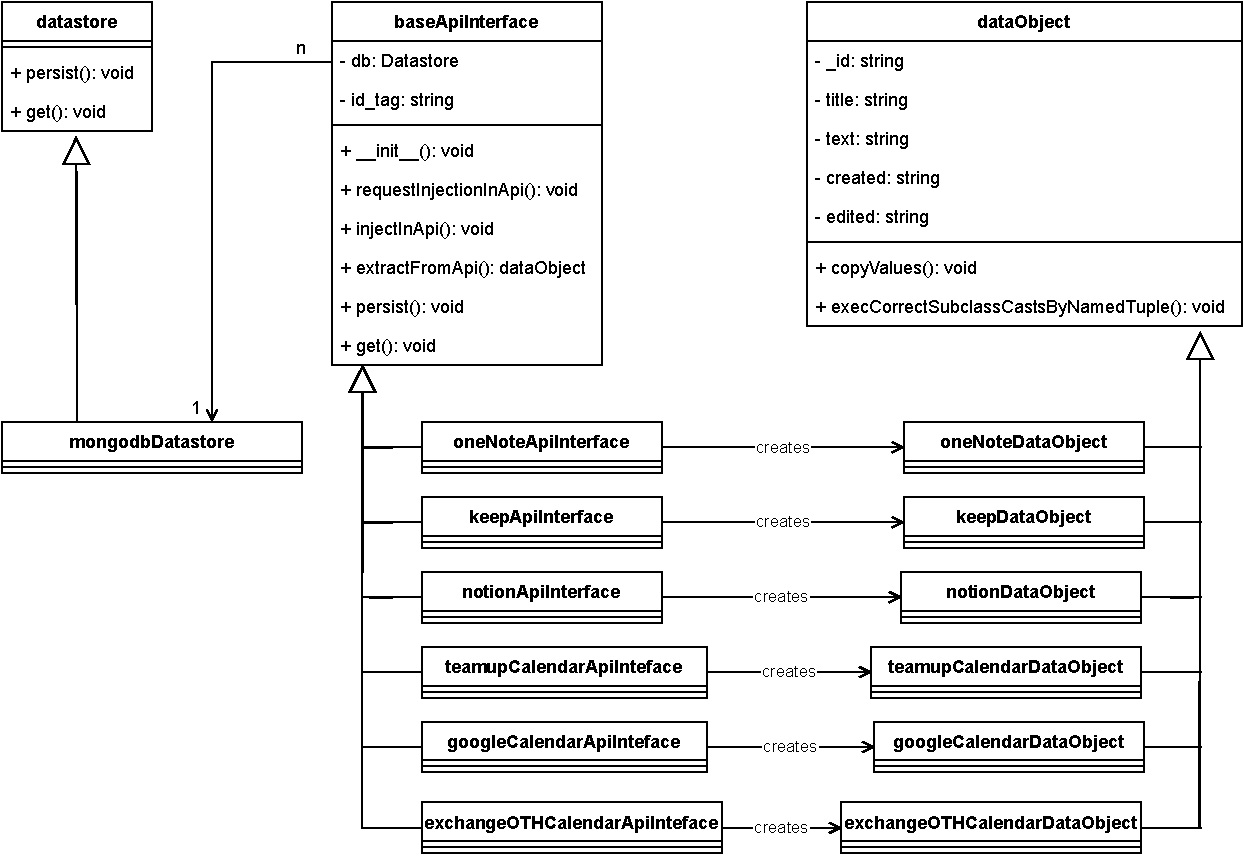
\includegraphics[width=1\textwidth]{Bilder/umsetzung/classDiagramm.pdf}
	\caption{Vereinfachtes Klassendiagramm zur Darstellung der Klassenstruktur}
	\label{fig:Klassendiagram}
\end{figure}

\section{Umsetzung des Speichervorganges}

\section{Definition des Extraktionsvorganges aus der Datenbank und der Datenrückführung in einen Dienst}